\documentclass{article}
\usepackage{tikz}
\usepackage{pgfplots}
\usetikzlibrary{shapes.geometric, arrows.meta, positioning, backgrounds}
\pgfplotsset{compat=1.17}

% Define colors
\definecolor{processblue}{RGB}{39, 87, 121}
\definecolor{processgreen}{RGB}{46, 139, 87}
\definecolor{processorange}{RGB}{255, 140, 0}
\definecolor{processred}{RGB}{220, 53, 69}

\begin{document}

% System Architecture Diagram
\begin{figure}[h]
\centering
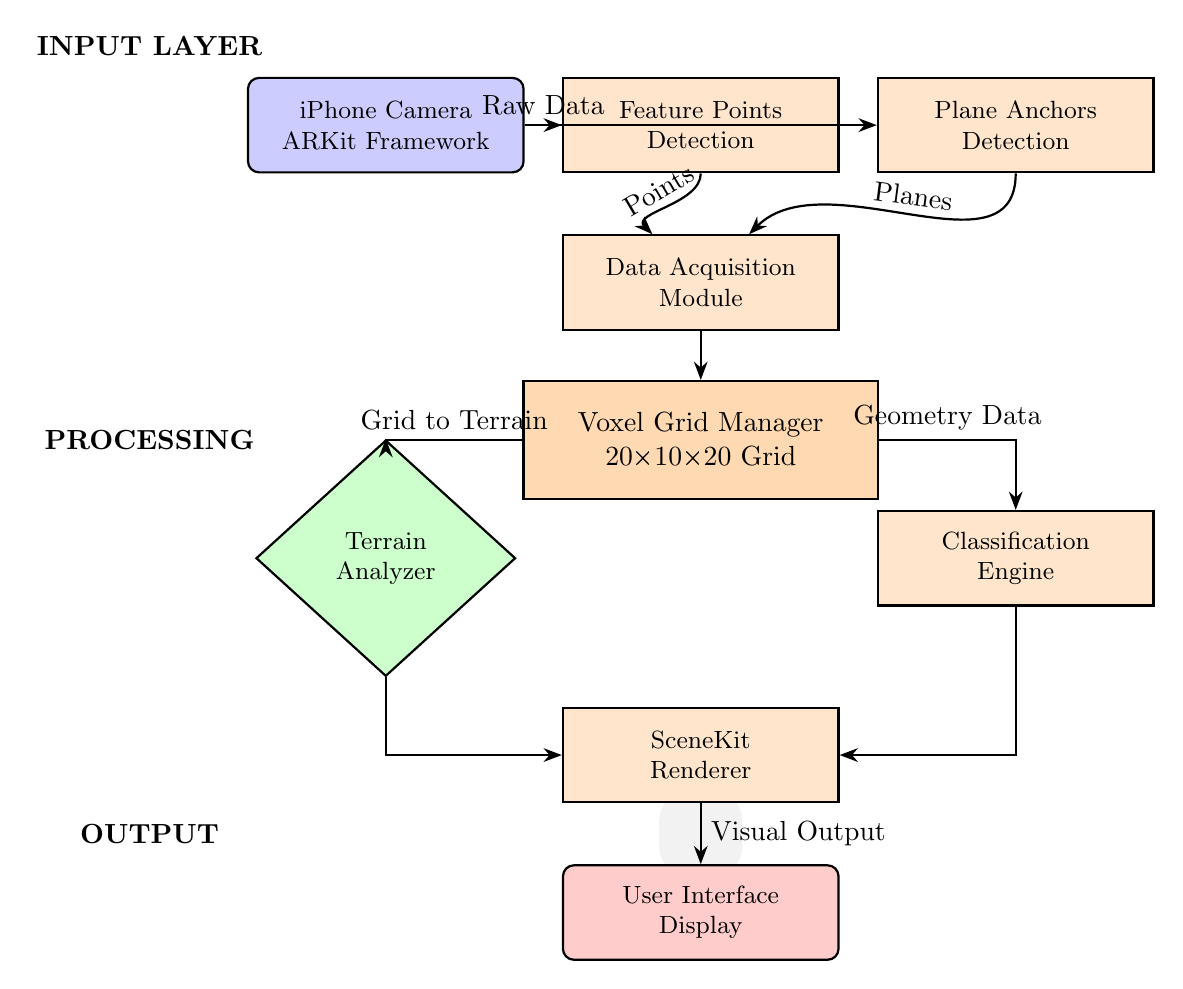
\begin{tikzpicture}[
    node distance = 2cm,
    input/.style = {rectangle, rounded corners, minimum width=3.5cm, minimum height=1.2cm, 
                    text centered, draw=black, fill=blue!20, font=\small, align=center, thick},
    process/.style = {rectangle, minimum width=3.5cm, minimum height=1.2cm, 
                      text centered, draw=black, fill=orange!20, font=\small, align=center, thick},
    bigprocess/.style = {rectangle, minimum width=4.5cm, minimum height=1.5cm, 
                         text centered, draw=black, fill=orange!30, font=\normalsize, align=center, thick},
    decision/.style = {diamond, aspect=2, minimum width=3cm, minimum height=3cm, 
                       text centered, draw=black, fill=green!20, font=\small, align=center, thick},
    output/.style = {rectangle, rounded corners, minimum width=3.5cm, minimum height=1.2cm, 
                     text centered, draw=black, fill=red!20, font=\small, align=center, thick},
    arrow/.style = {->, >=Stealth, thick},
    layer/.style = {fill=gray!10, rounded corners=10pt, inner sep=15pt, outer sep=5pt}
]

% Background layers - positioned further back
\begin{scope}[on background layer]
    \node[layer] (inputlayer) at (0, 5) {};
    \node[layer] (processlayer) at (0, 1) {};
    \node[layer] (outputlayer) at (0, -4) {};
\end{scope}

% Layer labels
\node[font=\bfseries] at (-7, 6) {INPUT LAYER};
\node[font=\bfseries] at (-7, 1) {PROCESSING};
\node[font=\bfseries] at (-7, -4) {OUTPUT};

% Nodes - Input Layer
\node (camera) [input] at (-4, 5) {iPhone Camera \\ ARKit Framework};
\node (features) [process] at (0, 5) {Feature Points \\ Detection};
\node (planes) [process] at (4, 5) {Plane Anchors \\ Detection};

% Nodes - Processing Layer
\node (acquisition) [process] at (0, 3) {Data Acquisition \\ Module};
\node (grid) [bigprocess] at (0, 1) {Voxel Grid Manager \\ 20×10×20 Grid};
\node (analyzer) [decision] at (-4, -0.5) {Terrain \\ Analyzer};
\node (classifier) [process] at (4, -0.5) {Classification \\ Engine};

% Nodes - Output Layer
\node (renderer) [process] at (0, -3) {SceneKit \\ Renderer};
\node (ui) [output] at (0, -5) {User Interface \\ Display};

% Arrows - Input to Processing
\draw [arrow] (camera) -- node[midway, above] {Raw Data} (features);
\draw [arrow] (camera) edge node[midway, above] {} (planes);

% Fixed arrows for Features and Planes to Acquisition - using curved paths and better positioning
\draw [arrow] (features) to[out=-90, in=135] node[midway, sloped, above] {Points} (acquisition);
\draw [arrow] (planes) to[out=-90, in=45] node[midway, sloped, above] {Planes} (acquisition);

% Arrows - Processing
\draw [arrow] (acquisition) -- (grid);
\draw [arrow] (grid) -| node[near start, above] {Grid to Terrain} (analyzer);
\draw [arrow] (grid) -| node[near start, above] {Geometry Data} (classifier);
\draw [arrow] (analyzer.south) |- (renderer);
\draw [arrow] (classifier.south) |- (renderer);

% Arrows - Output
\draw [arrow] (renderer) -- node[midway, right] {Visual Output} (ui);

\end{tikzpicture}
\caption{System Architecture Overview: Data flows from ARKit input through processing layers to voxel visualization}
\end{figure}

% Terrain Classification Accuracy Graph
\begin{figure}[h]
\centering
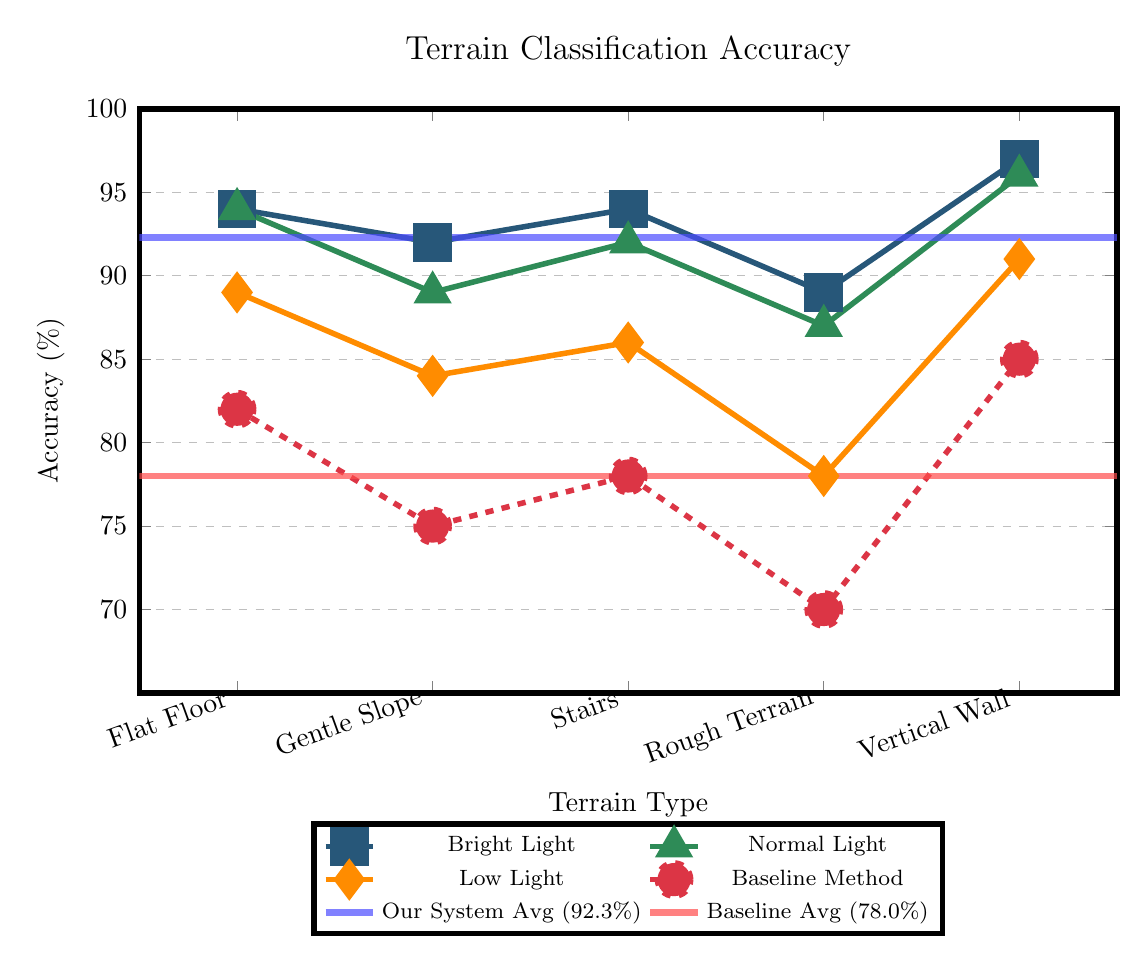
\begin{tikzpicture}
\begin{axis}[
    width=14cm,
    height=9cm,
    title style={font=\large, yshift=5pt},
    title={Terrain Classification Accuracy},
    xlabel={Terrain Type},
    ylabel={Accuracy (\%)},
    xmin=0.5, xmax=5.5,
    ymin=65, ymax=100,
    xtick={1,2,3,4,5},
    xticklabels={
        {Flat Floor},
        {Gentle Slope},
        {Stairs},
        {Rough Terrain},
        {Vertical Wall}
    },
    x tick label style={rotate=20, anchor=east},
    ytick={70,75,80,85,90,95,100},
    legend style={at={(0.5,-0.22)}, anchor=north, legend columns=2, font=\footnotesize},
    ymajorgrids=true,
    grid style=dashed,
    line width=2pt,
    mark size=6pt,
]

% Our System data - Different lighting conditions
\addplot[color=processblue, mark=square*] coordinates {
    (1,94) (2,92) (3,94) (4,89) (5,97)
};
\addlegendentry{Bright Light}

\addplot[color=processgreen, mark=triangle*] coordinates {
    (1,94) (2,89) (3,92) (4,87) (5,96)
};
\addlegendentry{Normal Light}

\addplot[color=processorange, mark=diamond*] coordinates {
    (1,89) (2,84) (3,86) (4,78) (5,91)
};
\addlegendentry{Low Light}

% Baseline method
\addplot[color=processred, mark=*, dashed] coordinates {
    (1,82) (2,75) (3,78) (4,70) (5,85)
};
\addlegendentry{Baseline Method}

% Average lines
\addplot[color=blue!70, line width=2.5, opacity=0.7] coordinates {
    (0.5,92.3) (5.5,92.3)
};
\addlegendentry{Our System Avg (92.3\%)}

\addplot[color=red!70, line width=2.5, opacity=0.7] coordinates {
    (0.5,78.0) (5.5,78.0)
};
\addlegendentry{Baseline Avg (78.0\%)}

\end{axis}
\end{tikzpicture}
\caption{Terrain Classification Accuracy: Performance metrics across different terrain types and lighting conditions}
\end{figure}

\end{document}